\documentclass[convert={size=768}]{standalone}
\usepackage[utf8]{inputenc}
\usepackage[T1]{fontenc}
\usepackage{amsmath}
\usepackage{amssymb}
\usepackage{tikz}
\usepackage{color}

\definecolor{draculaPurple}{RGB}{189,147,249}
\definecolor{draculaCyan}{RGB}{139,233,253}
\definecolor{draculaForeground}{RGB}{248,248,248}
\definecolor{draculaRed}{RGB}{255, 85, 85}

\begin{document}
	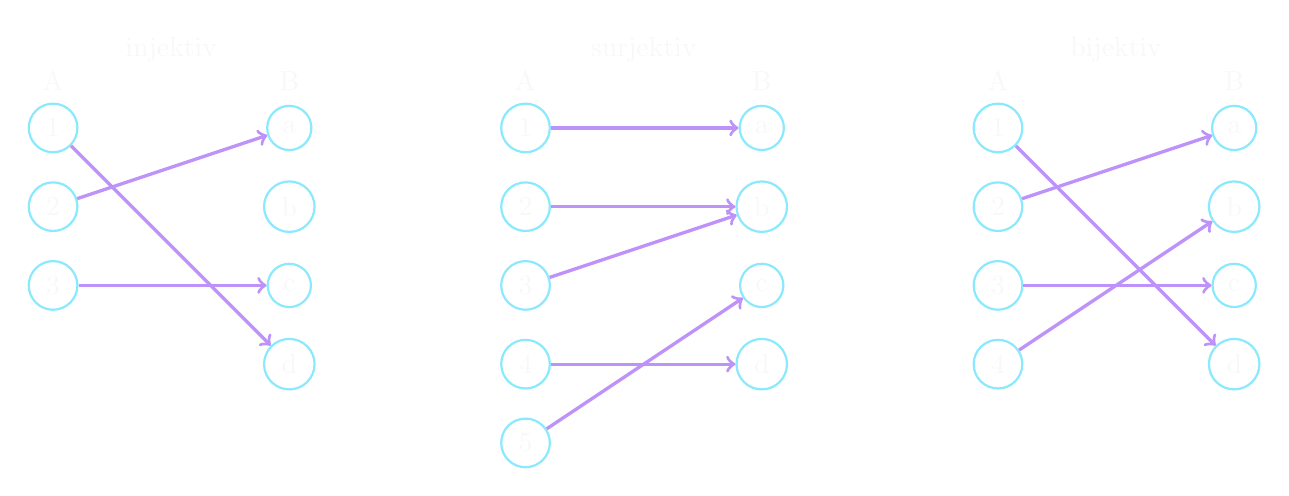
\begin{tikzpicture}[text=draculaForeground, draw=draculaCyan]
		% Injection
		% Set names
		\node at (1.5,0) [thick] {injektiv};
		\node at (0,-0.4) [thick] {A};
		\node at (3,-0.4) [thick] {B};
		
		% Set elements
		\begin{scope}[every node/.style={circle,thick,draw}]
			\node (1) at (0,-1) {1};
			\node (2) at (0,-2) {2};
			\node (3) at (0,-3) {3};
		\end{scope}
		\begin{scope}[every node/.style={circle,thick,draw}]
			\node (A) at (3,-1) {a};
			\node (B) at (3,-2) {b};
			\node (C) at (3,-3) {c};
			\node (D) at (3,-4) {d};
		\end{scope}
		
		% Arrows
		\begin{scope}[every edge/.style={draw=draculaPurple,very thick}]
			\path [->] (1) edge (D);
			\path [->] (2) edge (A);
			\path [->] (3) edge (C);
		\end{scope}
	
		% Surjection
		% Set names
		\node at (7.5,0) [thick] {surjektiv};
		\node at (6,-0.4) [thick] {A};
		\node at (9,-0.4) [thick] {B};
		
		% Set elements
		\begin{scope}[every node/.style={circle,thick,draw}]
			\node (11) at (6,-1) {1};
			\node (22) at (6,-2) {2};
			\node (33) at (6,-3) {3};
			\node (44) at (6,-4) {4};
			\node (55) at (6,-5) {5};
		\end{scope}
		\begin{scope}[every node/.style={circle,thick,draw}]
			\node (AA) at (9,-1) {a};
			\node (BB) at (9,-2) {b};
			\node (CC) at (9,-3) {c};
			\node (DD) at (9,-4) {d};
		\end{scope}
		
		% Arrows
		\begin{scope}[every edge/.style={draw=draculaPurple,very thick}]
			\path [->] (11) edge (AA);
			\path [->] (22) edge (BB);
			\path [->] (33) edge (BB);
			\path [->] (44) edge (DD);
			\path [->] (55) edge (CC);
		\end{scope}
		
		% Bijection
		% Set names
		\node at (13.5,0) [thick] {bijektiv};
		\node at (12,-0.4) [thick] {A};
		\node at (15,-0.4) [thick] {B};
		
		% Set elements
		\begin{scope}[every node/.style={circle,thick,draw}]
			\node (111) at (12,-1) {1};
			\node (222) at (12,-2) {2};
			\node (333) at (12,-3) {3};
			\node (444) at (12,-4) {4};
		\end{scope}
		\begin{scope}[every node/.style={circle,thick,draw}]
			\node (AAA) at (15,-1) {a};
			\node (BBB) at (15,-2) {b};
			\node (CCC) at (15,-3) {c};
			\node (DDD) at (15,-4) {d};
		\end{scope}
		
		% Arrows
		\begin{scope}[every edge/.style={draw=draculaPurple,very thick}]
			\path [->] (111) edge (DDD);
			\path [->] (222) edge (AAA);
			\path [->] (333) edge (CCC);
			\path [->] (444) edge (BBB);
		\end{scope}
	\end{tikzpicture}
\end{document}